% !TEX root = ../thesis.tex

\section{Results}
\label{sec:results}

% Results overview
The results of the search for a new heavy boson resonance are considered in terms of exclusion limits for the benchmark signal models described in this analysis.
These limits are model-independent, and cover spin-0, spin-1, and spin-2 resonances decaying to \WW, \WZ, and \WH.

\subsection{Asymptotic Limits and Quantifying Excess}

% Asymptotic limits
The exclusion limits obtained for the analysis are asymptotic frequentist limits for the production cross section times the branching fraction for each signal model.
These limits are obtained by using an asymptotic approximation of the distributions for a test statistic $\tilde{q}_\mu$ that is based on a profile likelihood ratio under signal and background hypotheses with signal strength $\mu$, where $\mu=0$ is the background-only model and $\mu=1$ is the nominal signal model~\cite{Cowan_2011,CMS-NOTE-2011-005}.

% Obtaining limits
The test statistic used is
\begin{equation}
  \tilde{q}_\mu=-2\ln\frac{\mathcal{L}(\mathrm{data}|\mu,\hat{\vb*{\theta}}_\mu)}{\mathcal{L}(\mathrm{data}|\hat{\mu},\hat{\vb*{\theta}})},\qquad 0\leq\hat{\mu}\leq\mu,
\end{equation}
where $\hat{\vb*{\theta}}_\mu$ corresponds to the conditional maximum likelihood estimators of the nuisance parameters $\vb*{\theta}$ for a specified signal strength $\mu$ and data, and $\hat{\mu}$ and $\hat{\vb*{\theta}}$ are the estimators for the global maximum of the likelihood.
After finding the observed test statistic $\tilde{q}_\mu^\mathrm{obs}$, we obtain the values of the nuisance parameters $\hat{\vb*{\theta}}_0^\mathrm{obs}$ and $\hat{\vb*{\theta}}_\mu^\mathrm{obs}$ to describe the data for the background-only and signal+background hypotheses, respectively.
We then generate toy MCs to construct the corresponding pdfs, $f(\tilde{q}_\mu|0,\hat{\vb*{\theta}}_0^\mathrm{obs})$ and $f(\tilde{q}_\mu|\mu,\hat{\vb*{\theta}}_\mu^\mathrm{obs})$.
These distributions are used to define two $p$-values associated with the background-only and signal+background hypotheses, which are denoted by $p_b$ and $p_\mu$, respectively.
The $p$-values are given by
\begin{equation}
  p_\mu=P(\tilde{q}_\mu\geq\tilde{q}_\mu^\mathrm{obs}|\operatorname{signal+background})=\int_{\tilde{q}_\mu^\mathrm{obs}}^\infty f(\tilde{q}_\mu|\mu,\hat{\vb*{\theta}}_\mu^\mathrm{obs})\dd{\tilde{q}_\mu},
\end{equation}
along with
\begin{equation}
  1-p_b=P(\tilde{q}_\mu\geq\tilde{q}_\mu^\mathrm{obs}|\operatorname{background-only})=\int_{\tilde{q}_0^\mathrm{obs}}^\infty f(\tilde{q}_\mu|0,\hat{\vb*{\theta}}_0^\mathrm{obs})\dd{\tilde{q}_\mu}.
\end{equation}
We then define the confidence-level (CL) upper limit $CL_s$ as
\begin{equation}
  CL_s=\frac{p_\mu}{1-p_b}.
\end{equation}
As an example, to obtain a 95\% confidence-level (CL) upper limit, we adjust $\mu$ until we obtain a value of $CL_s=0.05$.

\subsection{Observed Limits}

% Observed limits
We derive 95\% CL upper limits on the resonance production cross section times branching fraction to \WW, \WZ, or \WH as a function of the mass hypothesis \MX for a narrow resonance, and compare them to expected cross sections from the benchmark models where available.
The resulting limits are shown in figures~\ref{fig:limits_spin0}-\ref{fig:limits_spin2} for the spin-0, spin-1, and spin-2 signal models.
These limits are obtained for the combination of all 24 search categories, showing the observed and median expected limits with the 68\% and 95\% expected bands, along with the theoretical cross sections for each of the signal models.
By comparing the observed limits to the theoretical cross sections, we may set mass exclusion limits for each of the resonance models.

% Observed excesses and exclusion limits
For the observed limits, no significant excess in the \MX spectrum is observed anywhere in the search region for any of the signal models.
The largest deviations from the expected background occur for the \VBF spin-1 signals, both for the neutral and charged signal models.
These deviations occur at $1\unit{TeV}$, with the largest $p$-value occurring in the \VBF\WprtoWZ model with a local significance of $3.01\sigma$.
Comparing the observed limits to the theoretical cross sections, we find that for spin-0 resonances decaying to \WW, \ggF-produced Bulk Radions with masses below $3.1\unit{TeV}$ are excluded at the 95\% CL.
For spin-1 resonances of the HVT model B, \DY-produced \ZprtoWW resonances lighter than $4.0\unit{TeV}$, \WprtoWZ resonances lighter than $3.9\unit{TeV}$, and \WprtoWH resonances lighter than $4.0\unit{TeV}$ are all excluded at the 95\% CL.
Finally, for spin-2 resonances decaying to \WW, \ggF-produced Bulk Gravitons with masses below $1.8\unit{TeV}$ are excluded at the 95\% CL.

\begin{figure}[htbp]
  \centering
  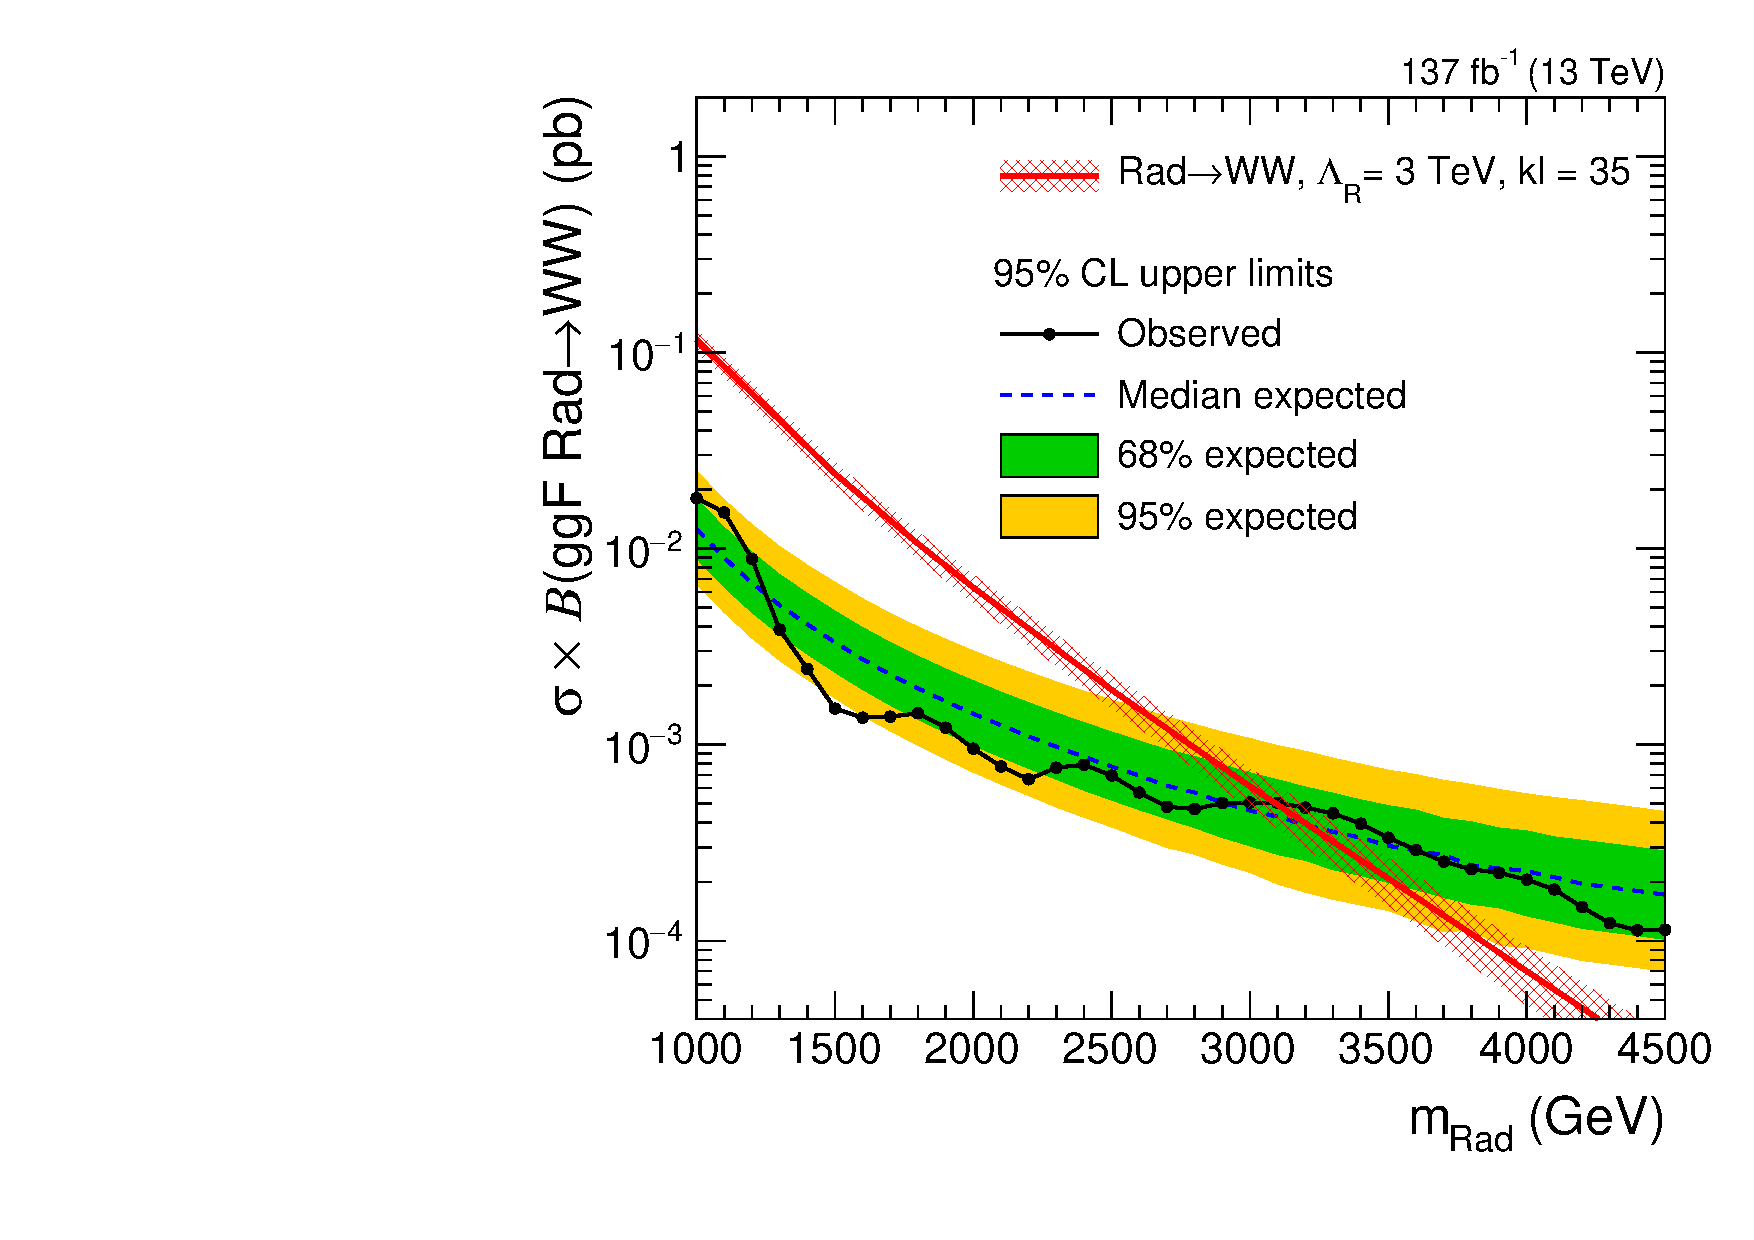
\includegraphics[width=0.4\textwidth]{fig/results/limits_RadToWW.pdf}
  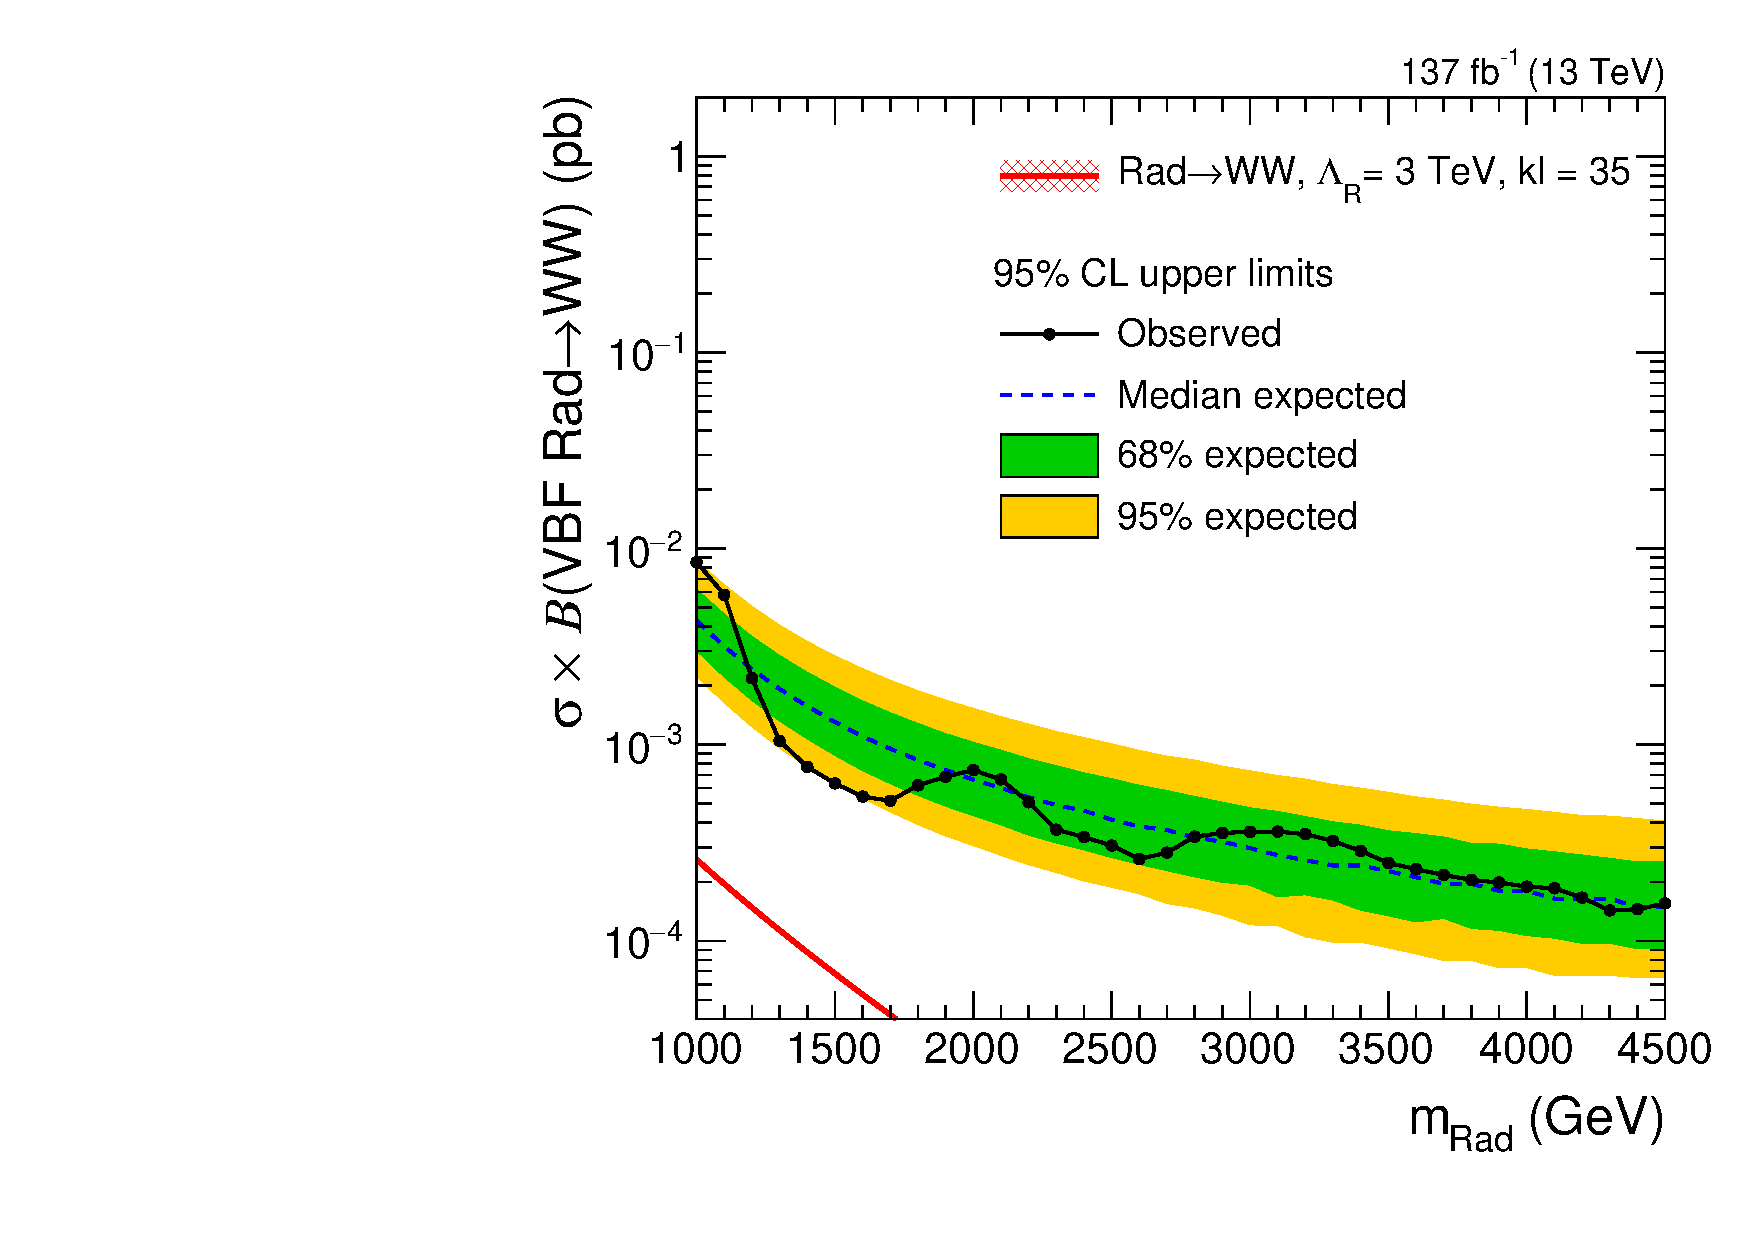
\includegraphics[width=0.4\textwidth]{fig/results/limits_VBFRadToWW.pdf}
  \caption{
    Exclusion limits for the production cross section times branching fraction for a new neutral spin-0 resonance produced via gluon-gluon fusion (left) or vector boson fusion (right) and decaying to \WW, as a function of the resonance mass hypothesis \MX, compared with the predicted cross sections for a spin-0 Bulk Radion with $\Lambda_{R}=3\unit{TeV}$ and $kl=35$.
    The signal cross section uncertainties are shown as red cross-hatched bands.
  }
  \label{fig:limits_spin0}
\end{figure}

\begin{figure}[htbp]
  \centering
  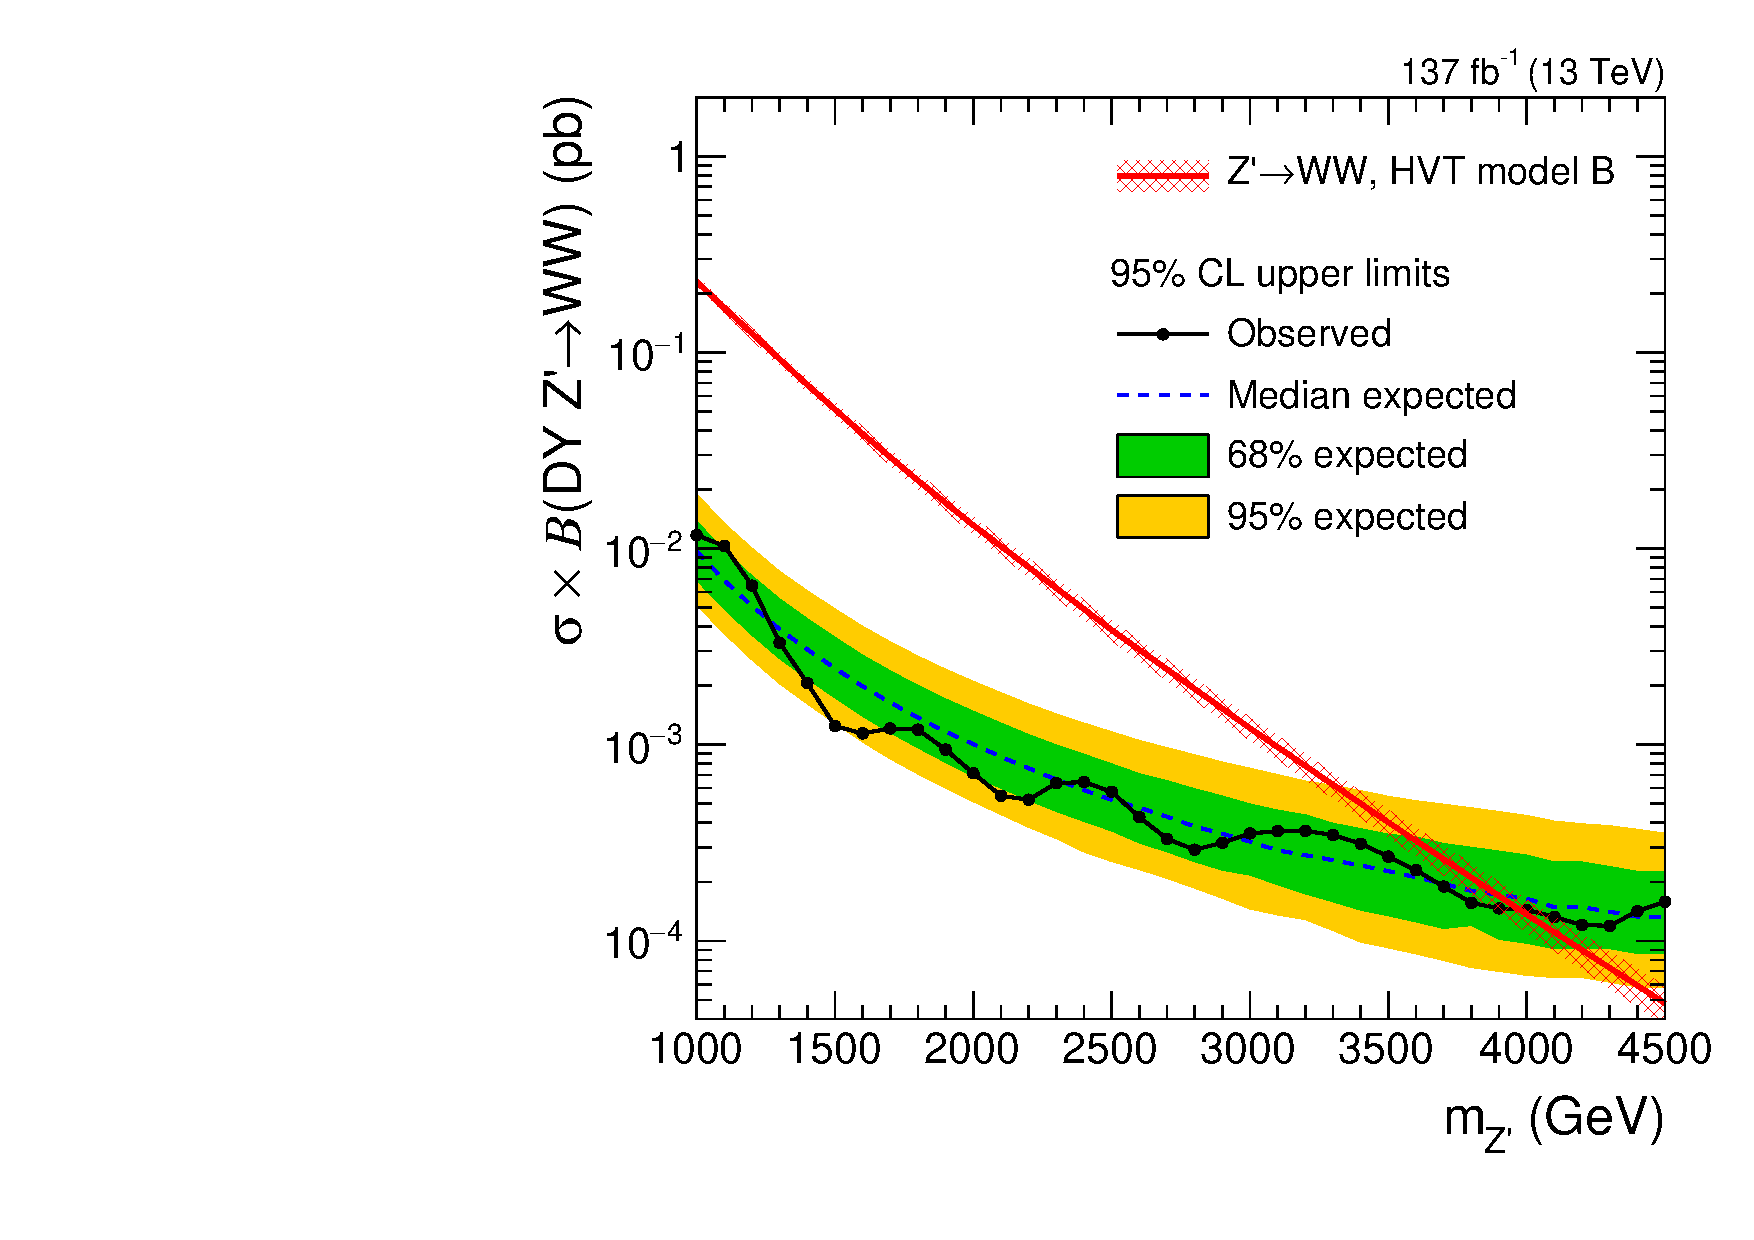
\includegraphics[width=0.4\textwidth]{fig/results/limits_ZprToWW.pdf}
  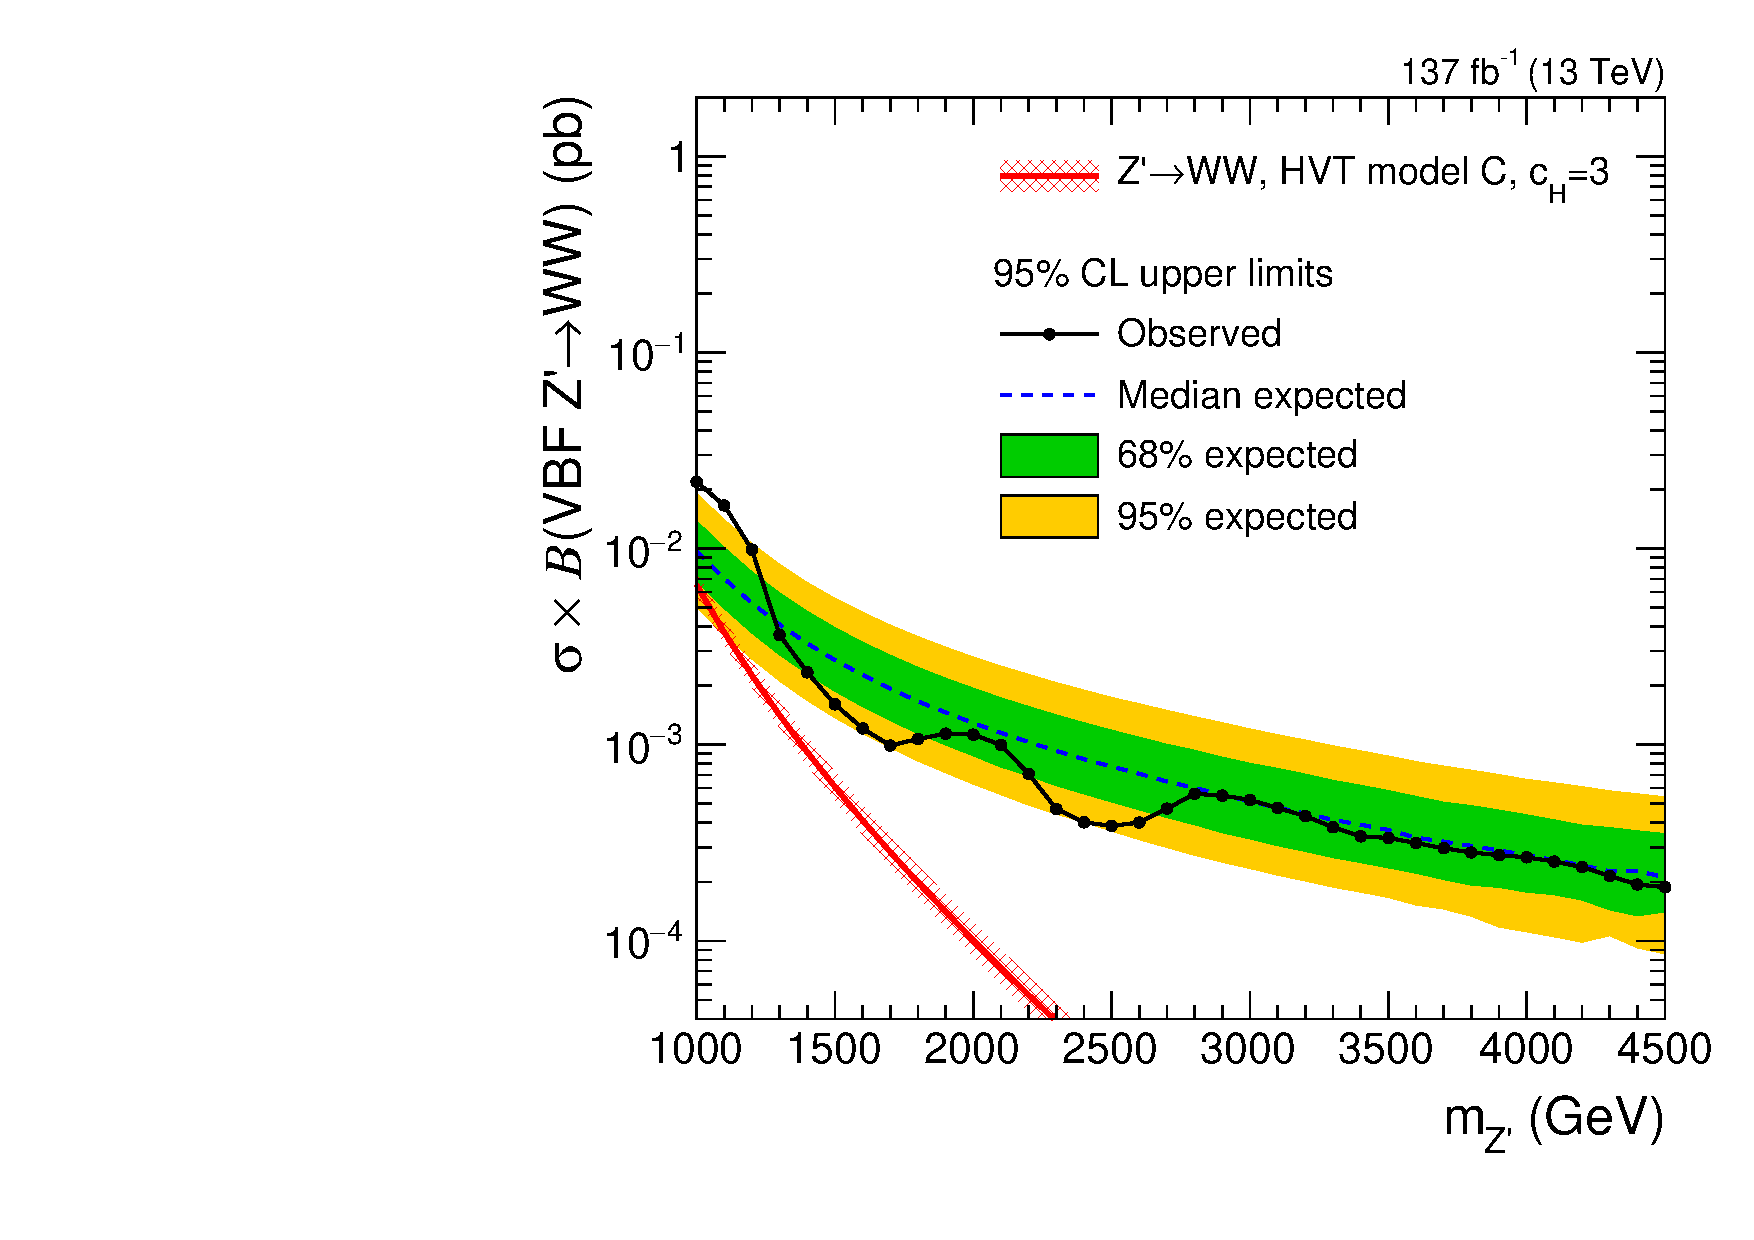
\includegraphics[width=0.4\textwidth]{fig/results/limits_VBFZprToWW.pdf}
  \caption{
    Exclusion limits for the production cross section times branching fraction for a new neutral spin-1 resonance produced via Drell-Yan (left) or vector boson fusion (right) and decaying to \WW, as a function of the resonance mass hypothesis \MX, compared with the predicted cross sections for a \Zpr from HVT model B (for \DY) or HVT model C with $c_\mathrm{H}=3$ (for \VBF).
    The signal cross section uncertainties are shown as red cross-hatched bands.
  }
  \label{fig:limits_spin1_neut}
\end{figure}

\begin{figure}[htbp]
  \centering
  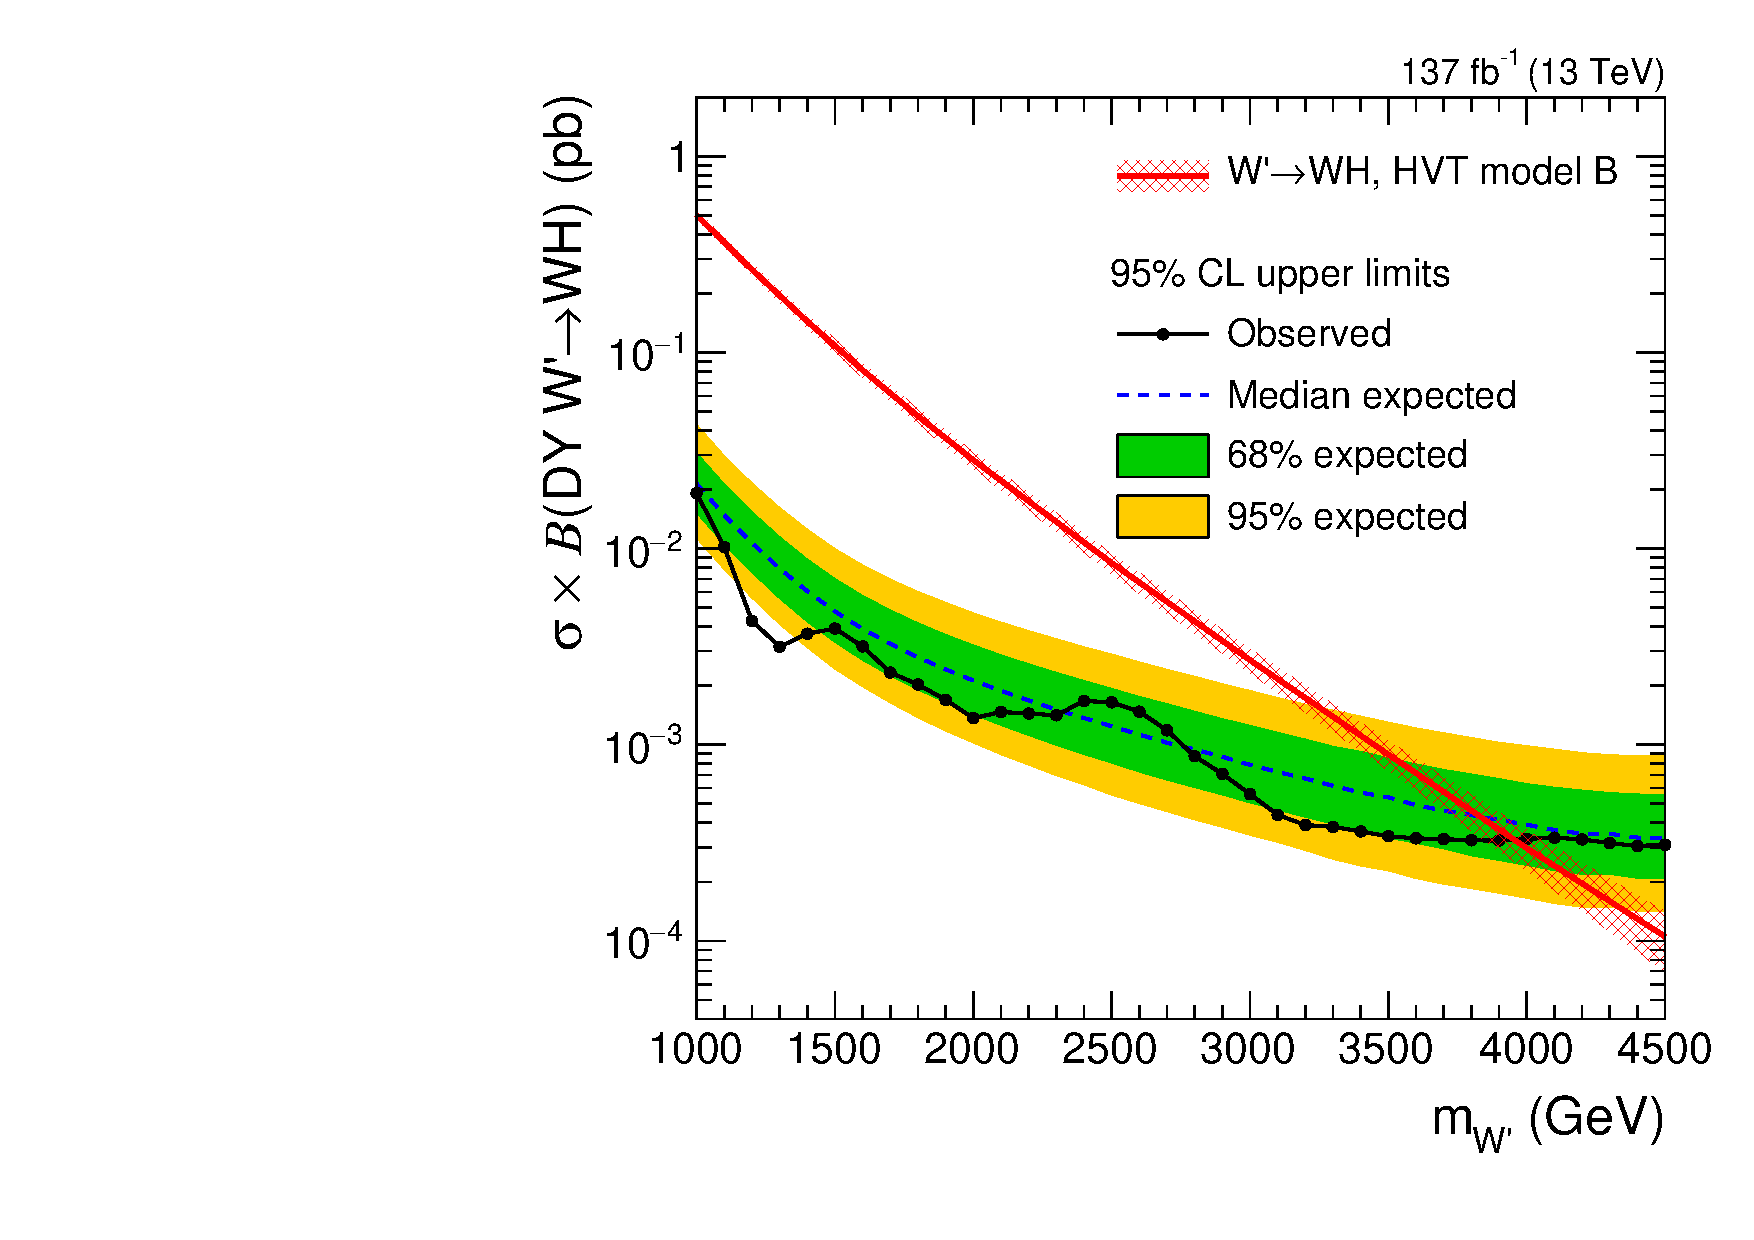
\includegraphics[width=0.4\textwidth]{fig/results/limits_WprToWH.pdf}
  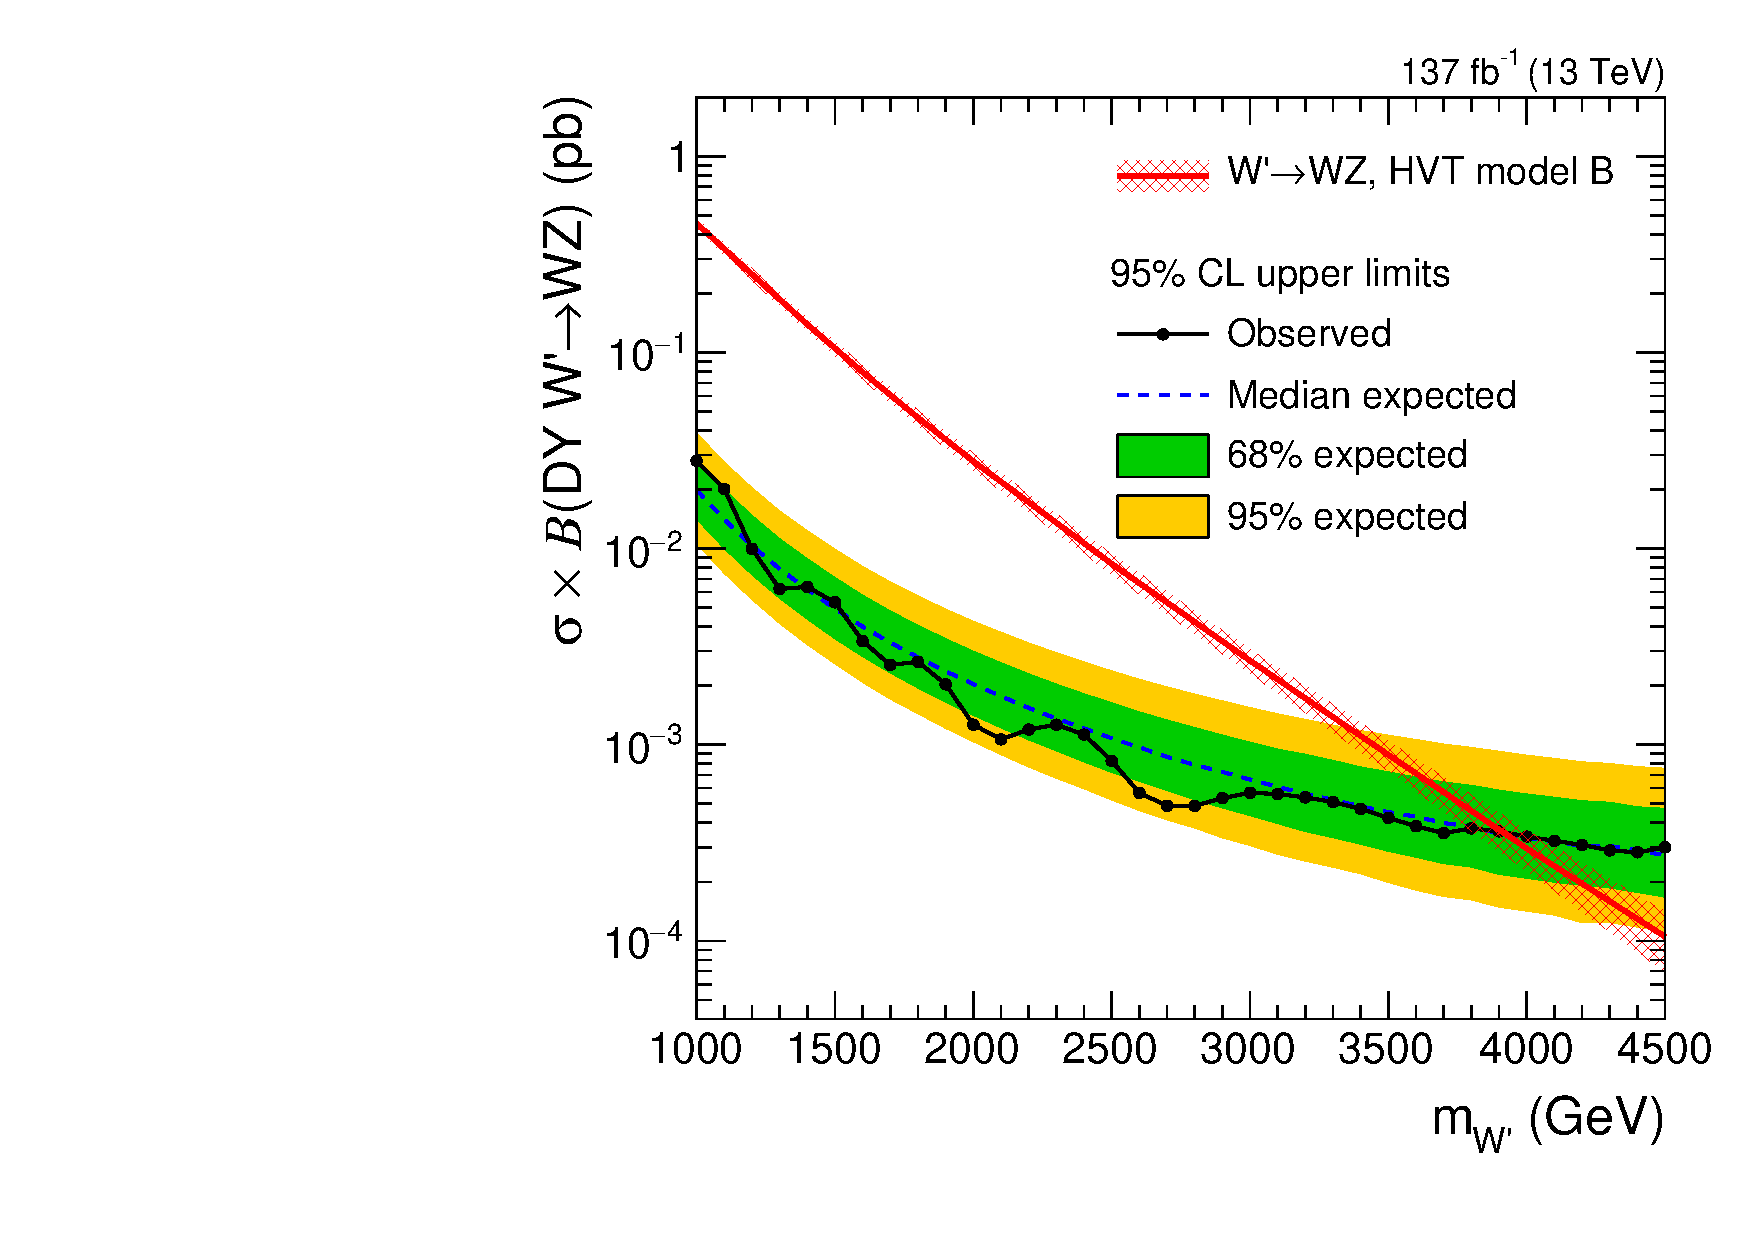
\includegraphics[width=0.4\textwidth]{fig/results/limits_WprToWZ.pdf}\\
  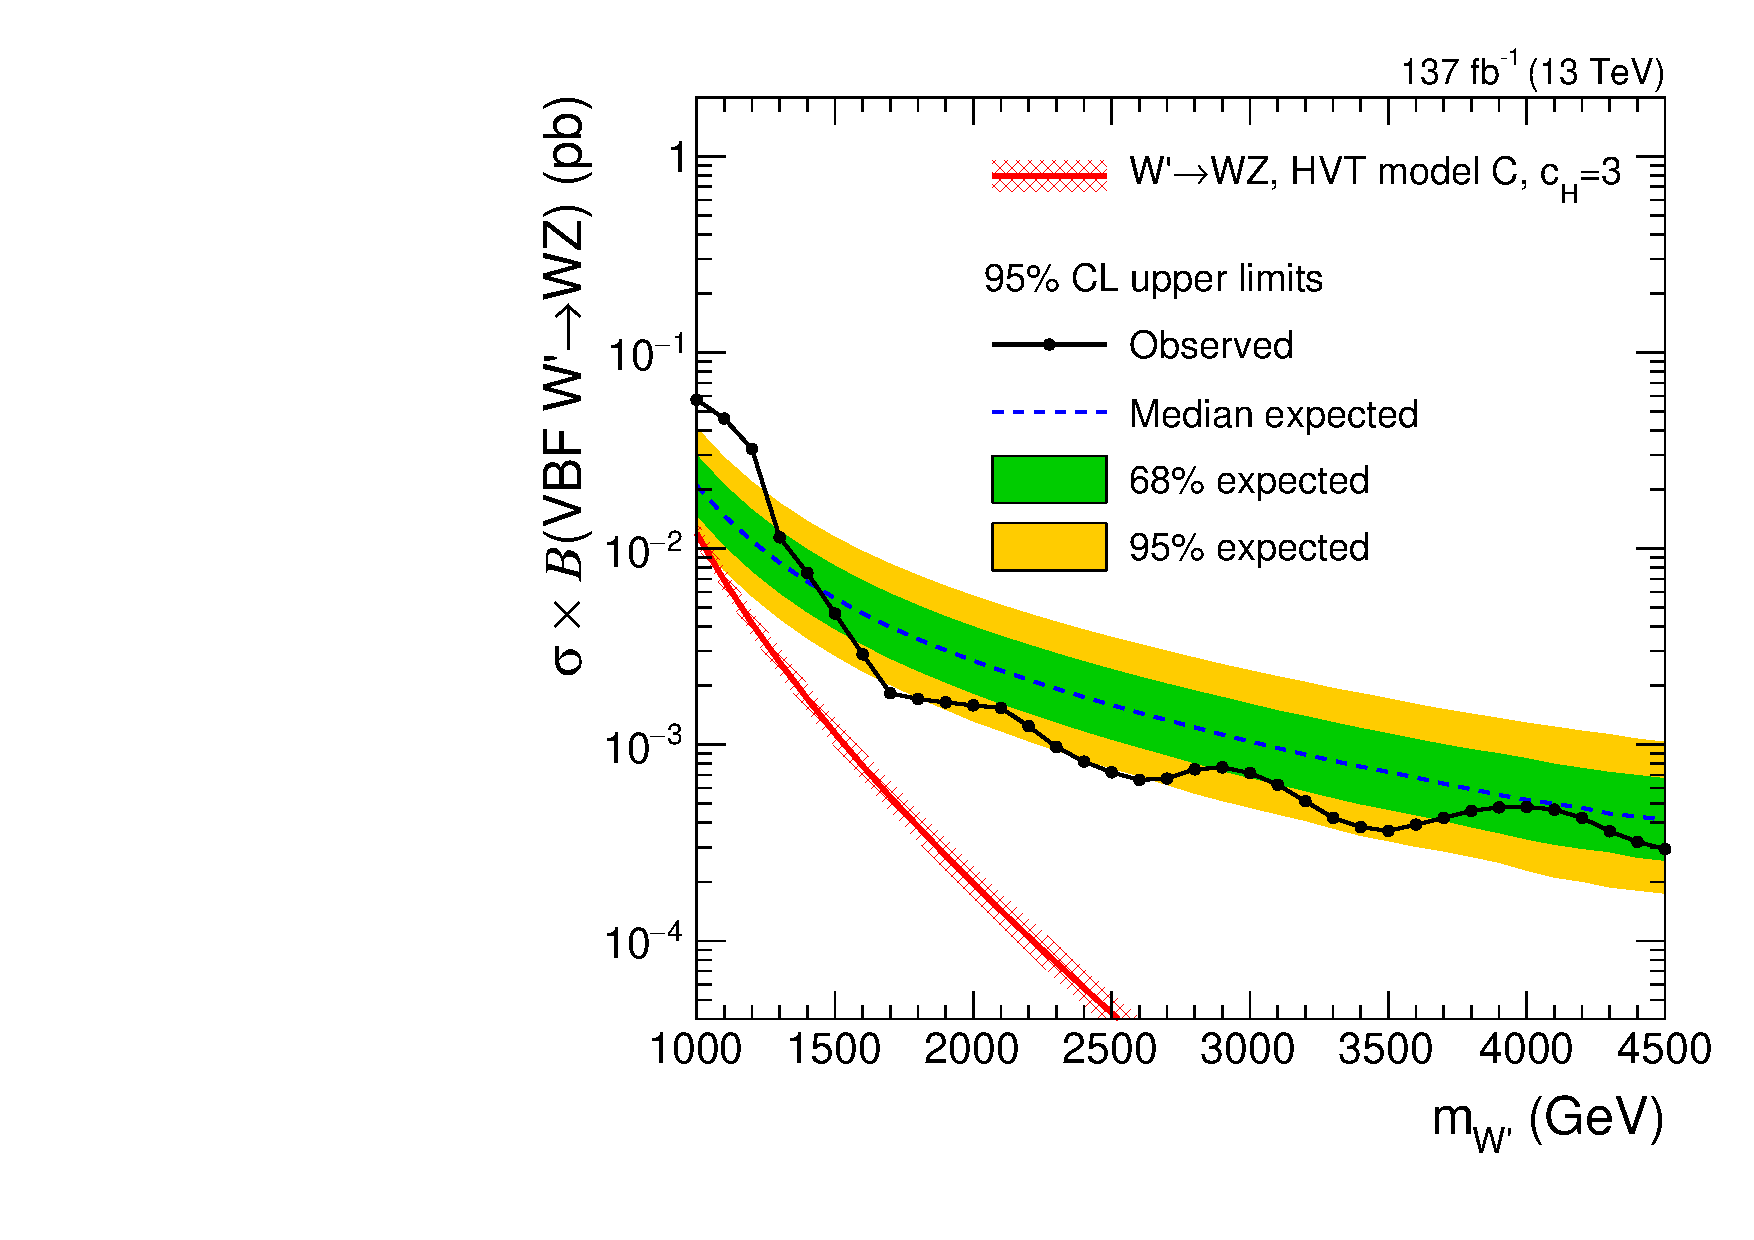
\includegraphics[width=0.4\textwidth]{fig/results/limits_VBFWprToWZ.pdf}
  \caption{
    Exclusion limits for the production cross section times branching fraction for a new charged spin-1 resonance produced via Drell-Yan (top left) and decaying to \WH, and for a new charged spin-1 resonance produced via Drell-Yan (top right) or vector boson fusion (bottom) and decaying to \WZ, as a function of the resonance mass hypothesis \MX, compared with the predicted cross sections for a \Wpr from HVT model B (for \DY) or HVT model C with $c_\mathrm{H}=3$ (for \VBF).
    The signal cross section uncertainties are shown as red cross-hatched bands.
  }
  \label{fig:limits_spin1_char}
\end{figure}

\begin{figure}[htbp]
  \centering
  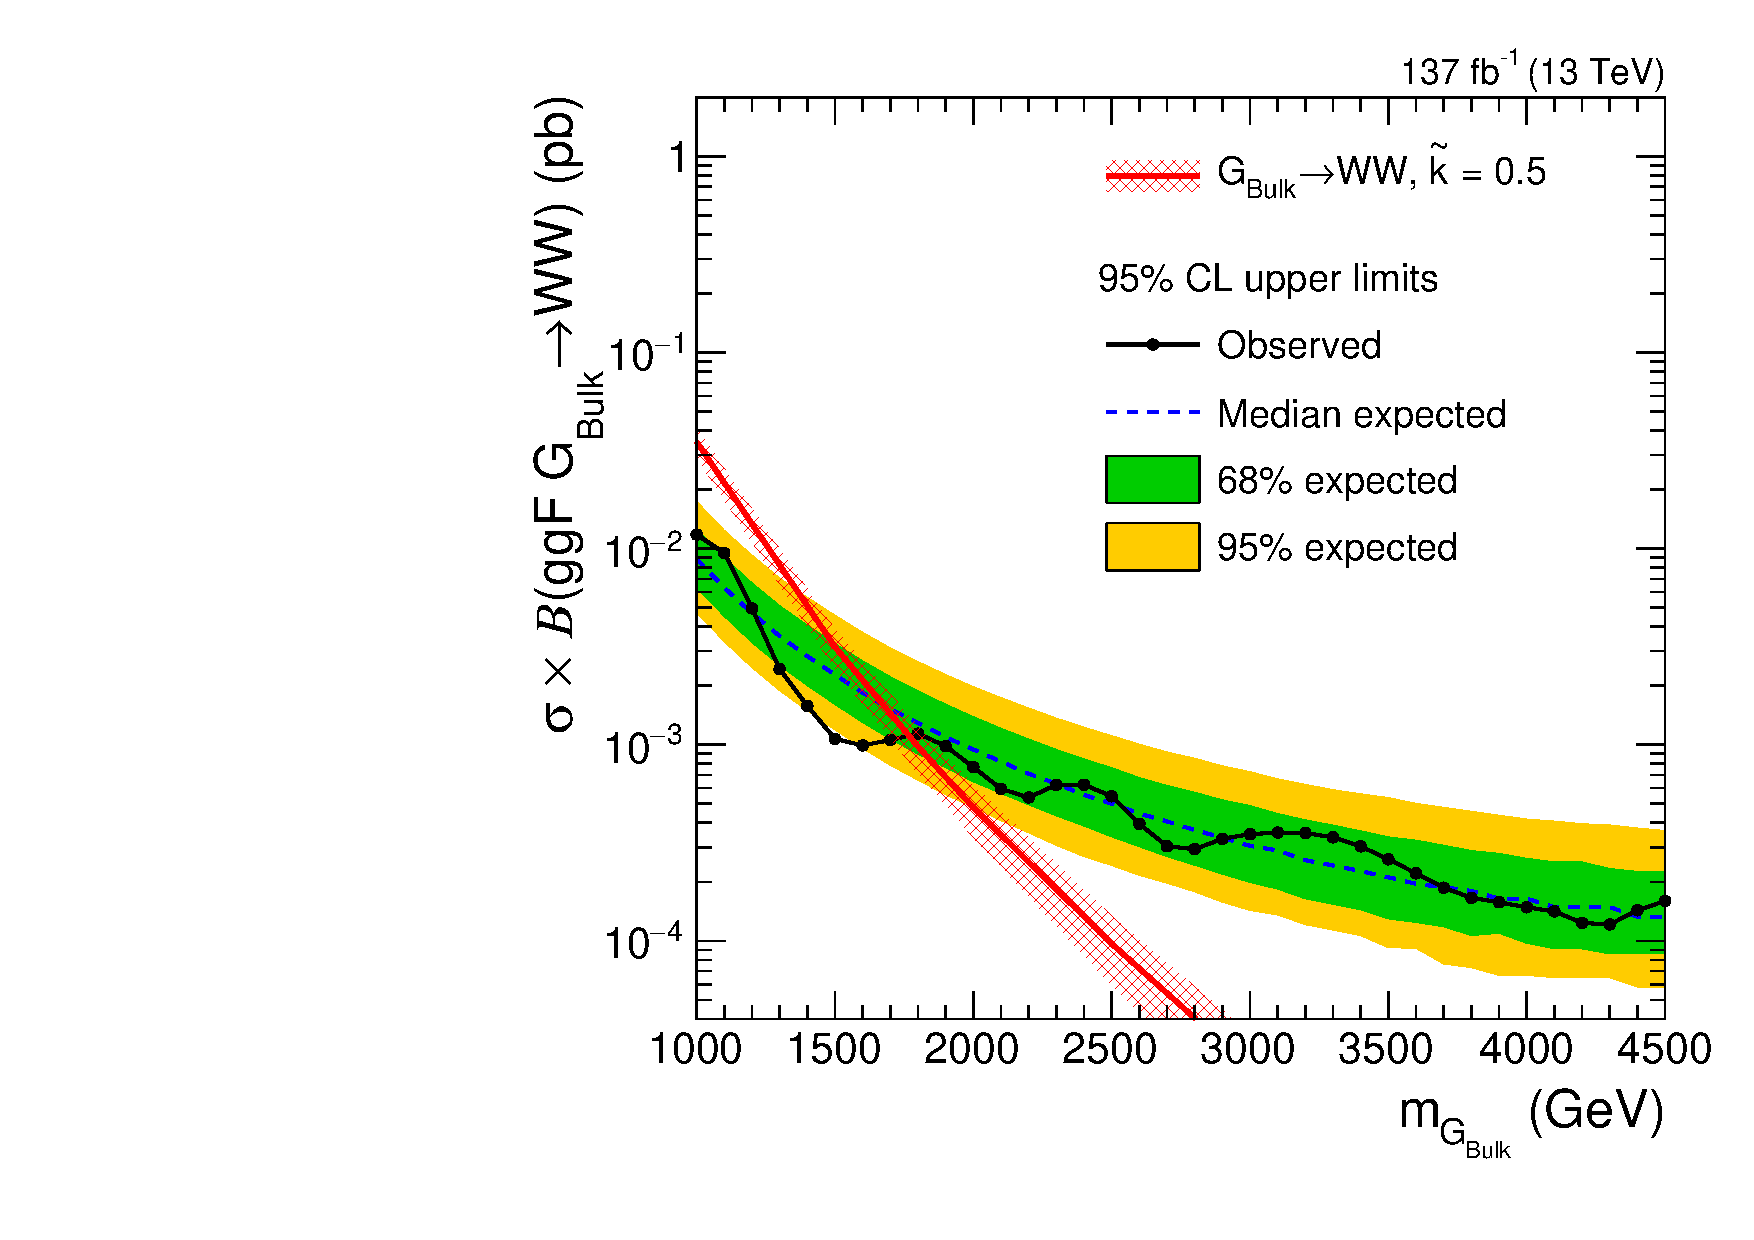
\includegraphics[width=0.4\textwidth]{fig/results/limits_GbuToWW.pdf}
  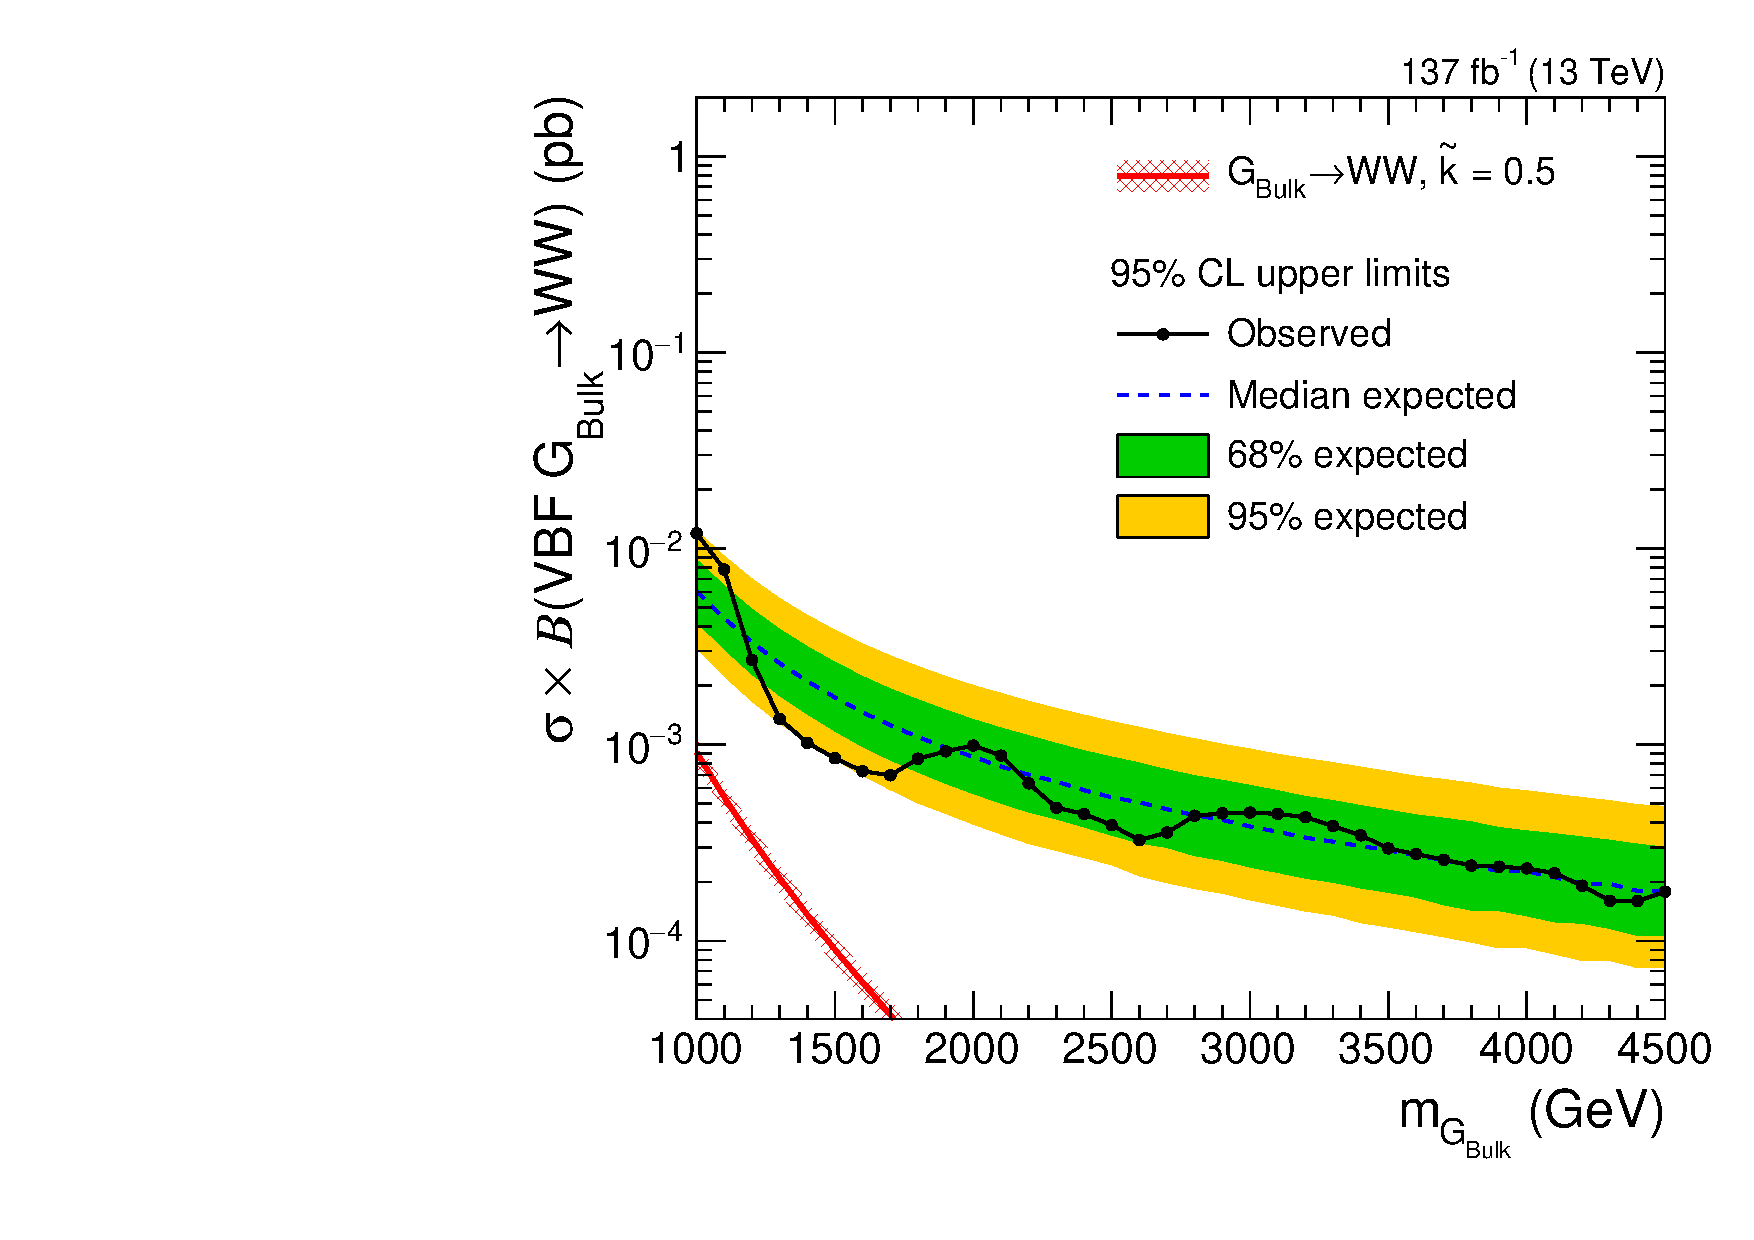
\includegraphics[width=0.4\textwidth]{fig/results/limits_VBFGbuToWW.pdf}
  \caption{
    Exclusion limits for the production cross section times branching fraction for a new neutral spin-2 resonance produced via gluon-gluon fusion (left) or vector boson fusion (right) and decaying to \WW, as a function of the resonance mass hypothesis \MX, compared with the predicted cross sections for a \GBulk with curvature $\tilde{k}=0.5$.
    The signal cross section uncertainties are shown as red cross-hatched bands.
  }
  \label{fig:limits_spin2}
\end{figure}
